\documentclass[problem]{mcs}

\begin{pcomments}
  \pcomment{FP_probability_relations_short_answer}
  \pcomment{ARM 12/14/15} 
    \pcomment{borrows from other short_answer problems,
      MQ_chains_and_antichains_sched, MQ_task_parallel_scheduling_v3}
\end{pcomments}

\pkeywords{
  equivalence
  partial_order
  DAG
  schedule
}

%%%%%%%%%%%%%%%%%%%%%%%%%%%%%%%%%%%%%%%%%%%%%%%%%%%%%%%%%%%%%%%%%%%%%
% Problem starts here
%%%%%%%%%%%%%%%%%%%%%%%%%%%%%%%%%%%%%%%%%%%%%%%%%%%%%%%%%%%%%%%%%%%%%

\begin{problem} For each of the relations described below, write the letters
\textbf{E, P, T, S, A, N} indicating which properties it has.

\begin{itemize}
\item an equivalence relation \hfill (\textbf{E}), 
\item a weak or strict partial order \hfill (\textbf{P}),
\end{itemize}
and if it is neither of the above, 
\begin{itemize}
\item \emph{transitive} \hfill (\textbf{T}),
\item \emph{symmetric} \hfill (\textbf{S}),
\item \emph{asymmetric} \hfill (\textbf{A}),
\item none of these  \hfill (\textbf{N}).
\end{itemize}

\medskip The relations on real-values random variables $R,S$:

\bparts

\ppart $\prob{R = S} = 1$. \hfill \examrule
\begin{solution} \textbf{E} \end{solution}

\ppart $\prob{R = S} = 0$. \hfill \examrule
\begin{solution} \textbf{S} \end{solution}

\ppart $\prob{R >0} = \pr{S > 0}$. \hfill \examrule
\begin{solution} \textbf{E} \end{solution}

\ppart $\expect{R} = \expect{S}$. \hfill \examrule
\begin{solution} \textbf{E} \end{solution}

\ppart $\expect{R} < \expect{S}$. \hfill \examrule
\begin{solution} \textbf{P} \end{solution}

\ppart $\expect{R} \neq \expect{S}$. \hfill \examrule
\begin{solution} \textbf{S} \end{solution}

\eparts

\medskip

The DAG in Figure~\ref{fig:taskdag8} shows the scheduling constraints
on a set of 8 tasks, each requiring unit time.

\begin{figure}
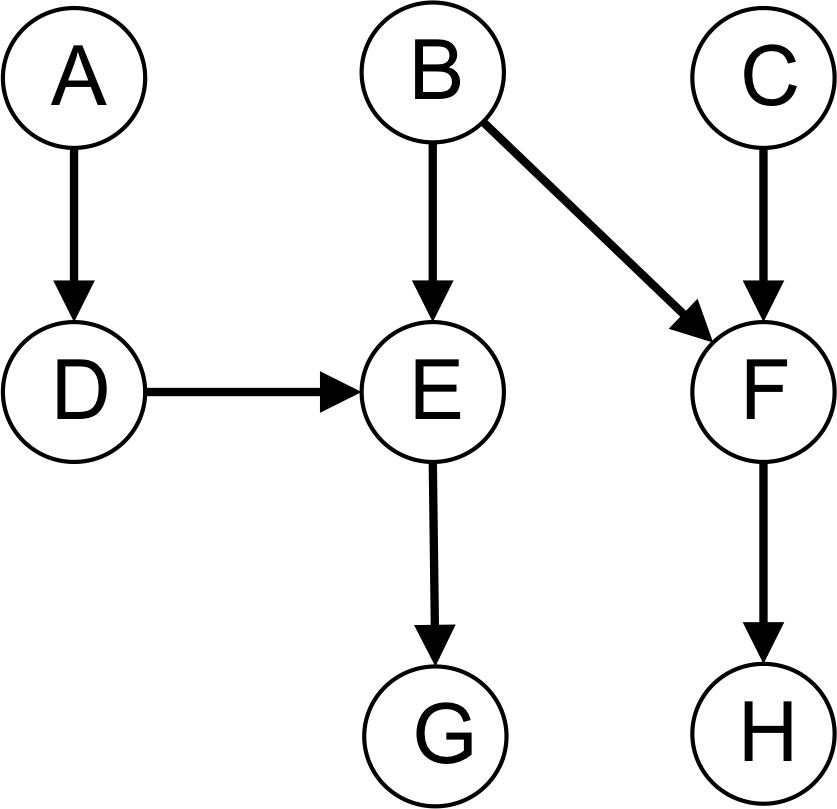
\includegraphics[height=1in]{miniquiz5-p2}
\caption{Task DAG}
\label{fig:taskdag8}
\end{figure}

\bparts

\ppart What is the minimum time required to complete all the tasks?
 \hfill \examrule

\begin{solution}
\textbf{4.}  This is the length of the longest chain.
\end{solution}

\ppart What is the minimum number of processors required to complete\\
all the tasks in minimum time?  \hfill \examrule
\begin{solution}
\textbf{2.}

Schedule $A,B$ then $C,D$ then $E,F$ then $G,H$.
\end{solution}

\eparts

\end{problem}

\endinput
